\documentclass{beamer}

\usepackage{polski}
\usepackage[T1]{fontenc}
\usepackage[utf8]{inputenc}

\usepackage[polish]{babel}

\usepackage{subfig}
\usepackage{rotating}

\usetheme[backgroundimagefile=bak.png,opacity=0.6]{diepen}

\title{Symulacja układu planetarnego na GPU przy użyciu CUDA i OpenGL}
\subtitle{część druga}
\author{Daniel Kłobuszewski\and Jakub Kotur}
\institute{{\normalsize Promotor: Krzysztof Kaczmarski}\\\vspace{1cm} Politechnika Warszawska}
\date{\today}

\begin{document}

\frame[plain]{\titlepage}

\frame
{
	\frametitle{Treść prezentacji}
	\tableofcontents
}

\section{Silnik graficzny}\label{sec:silnik graficzny}

\frame
{
	\frametitle{Shadery}
	\begin{figure}
	\centering
		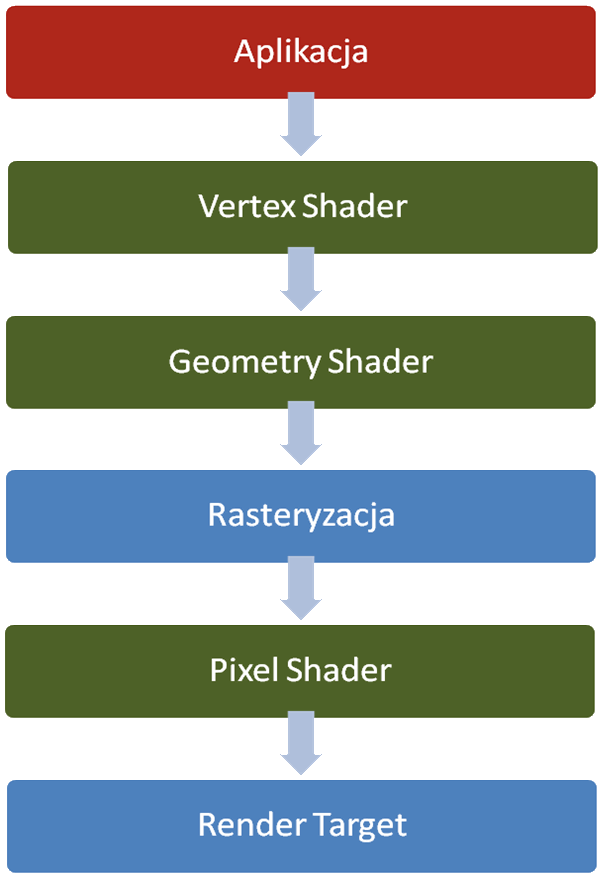
\includegraphics[height=7cm]{img/potok.png}
	\end{figure}
	\setcounter{subfigure}{0}
}

\frame
{
	\frametitle{Konstrukcja silnika}

	\begin{enumerate}
	\item Zbieranie danych do bufora geometrii
		\begin{enumerate}
		\item Generowanie geometrii
		\item Zbieranie danych o materiale
		\item Teksturowanie (kolor)
		\end{enumerate}
	\item Wyświetlanie finalnego obrazu
		\begin{enumerate}
		\item Obliczanie oświetlenia
		\end{enumerate}
	\end{enumerate}
}

\frame
{
	\frametitle{Potrzebne dane}

	W każdym pikselu potrzebna jest informacja:

	\begin{itemize}
	\item pozycja 
	\item normalna
	\item kolor
	\item materiał
	\end{itemize}
}

\begin{frame}[fragile]
	\frametitle{Reprezentacja danych}

	\begin{verbatim}
 buffers   |          values 
-----------+--------+--------+--------+----------
 texture 1 | pos.x  | pos.y  | pos.z  | alpha
 texture 2 | norm.x | norm.y | norm.z | acol.r
 texture 3 | col.r  | col.g  | col.b  | acol.g   
 texture 4 | ke     | ka     | kd     | acol.b
	\end{verbatim}
\end{frame}

\frame
{
	\frametitle{Wydajność}

	Teoretyczna maksymalna wydajność dla karty geforce 9800GTX przy rozdzielczości full hd (1920x1080):

	$$ Buffor size = 1920 \cdot 1080 \cdot 4 \cdot 4B \simeq 32MB $$

	\pause

	$$ \frac{Bandwidth}{Buffor size} = \frac{70GB/s}{32MB} = 2240 fps $$
}

\frame
{
	\frametitle{Źródła danych}

	Dane stałe dla planety:

	\begin{itemize}
	\item kolor planety
	\item materiał
	\end{itemize}

	Dane różne w każdym pikselu:

	\begin{itemize}
	\item pozycja 
	\item normalna
	\end{itemize}
}

\subsection{Geometria}\label{sub:geometria}
\frame{ \frametitle{Silnik graficzny} \tableofcontents[currentsubsection] }

\frame
{
	\frametitle{Geometria}

	\begin{enumerate}
	\item wygenerowanie mapy normalnych
	\item wyświetlenie kwadratu
	\item oteksturowanie kwadratu mapą normalnych
	\item normalne są przepisywane
	\item pozycja jest liczona z środka planety, normalnej i promienia
	\end{enumerate}
}

\frame
{
	\frametitle{Mapa normalnych}
	
	$$ (r,g,b) = (x,y,z) $$

	\begin{figure}
	\centering
	\caption{Mapa normalnych}
	\subfloat[]{\label{fig:normq}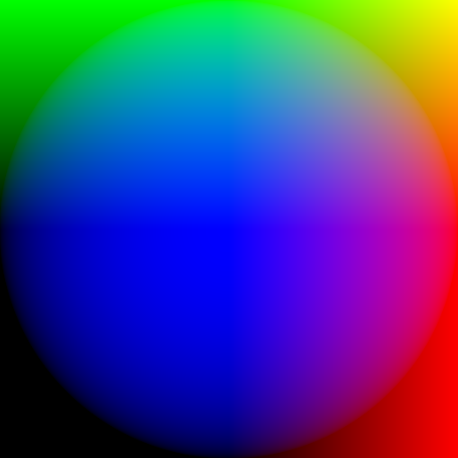
\includegraphics[width=0.4\textwidth]{img/norm_quad.png}} \hspace{.0\textwidth}
	\pause
	\subfloat[]{\label{fig:norms}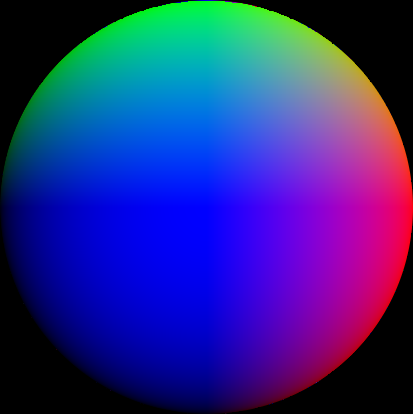
\includegraphics[width=0.4\textwidth]{img/norm_sphere.png}}
	\label{fig:normmap}
	\end{figure}
	\setcounter{subfigure}{0}
}

\frame
{
	\frametitle{Punkty}
	\begin{figure}
	\centering
		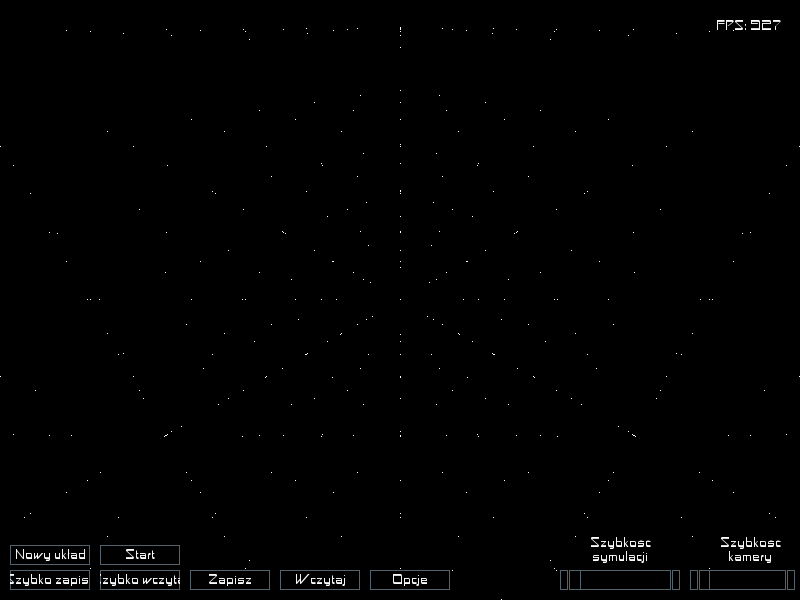
\includegraphics[height=7cm]{img/orto1.png}
	\label{fig:orto1}
	\end{figure}
	\setcounter{subfigure}{0}
}

\frame
{
	\frametitle{Kwadraty}
	\begin{figure}
	\centering
		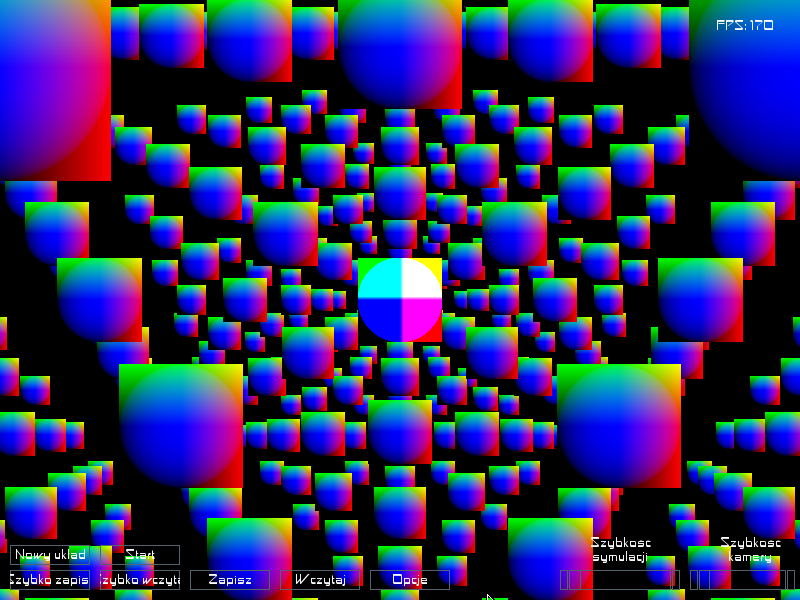
\includegraphics[height=7cm]{img/orto2.png}
	\label{fig:orto2}
	\end{figure}
	\setcounter{subfigure}{0}
}

\frame
{
	\frametitle{Koła}
	\begin{figure}
	\centering
		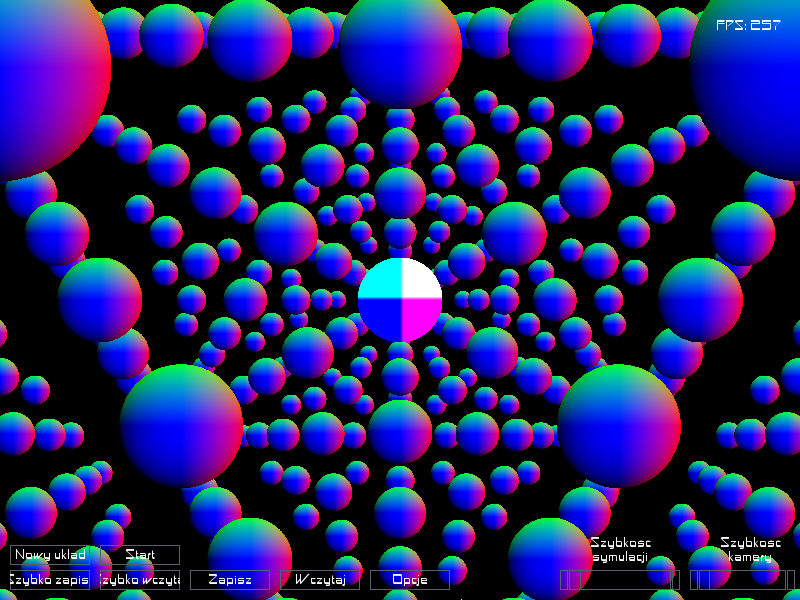
\includegraphics[height=7cm]{img/orto3.png}
	\label{fig:orto3}
	\end{figure}
}

\frame
{
	\frametitle{Rzut perspektywiczny}
	\begin{figure}
	\centering
		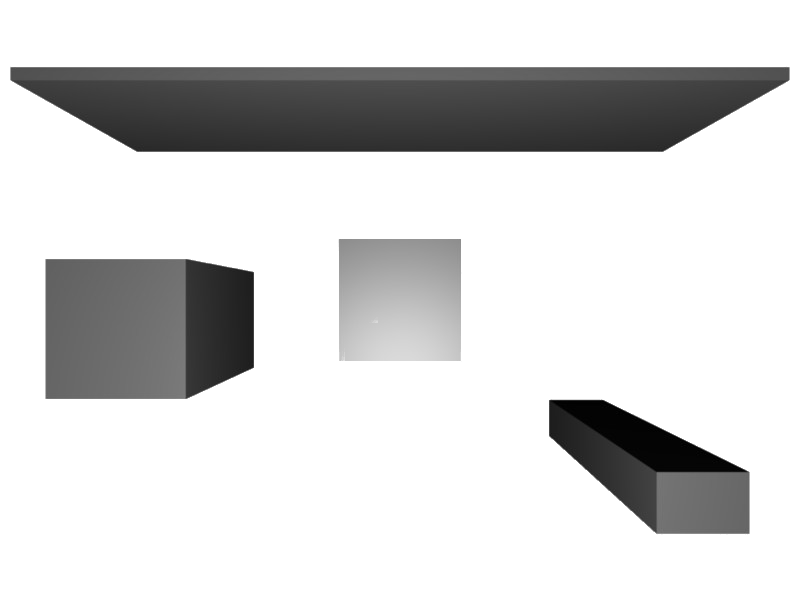
\includegraphics[height=7cm]{img/per_cube.png}
	\label{fig:perc}
	\end{figure}
}

\frame
{
	\frametitle{Kwadraty - perspektywa}
	\begin{figure}
	\centering
		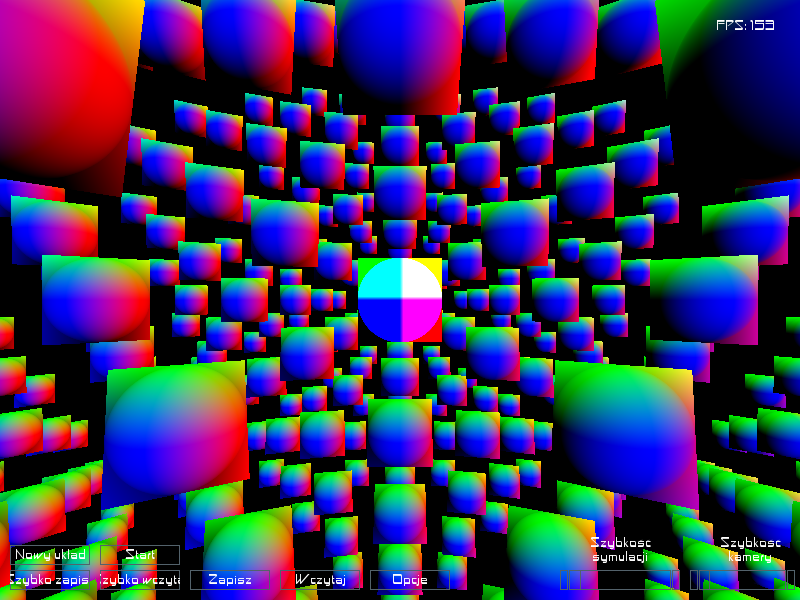
\includegraphics[height=7cm]{img/per1.png}
	\label{fig:per1}
	\end{figure}
}

\frame
{
	\frametitle{Koła - perspektywa}
	\begin{figure}
	\centering
		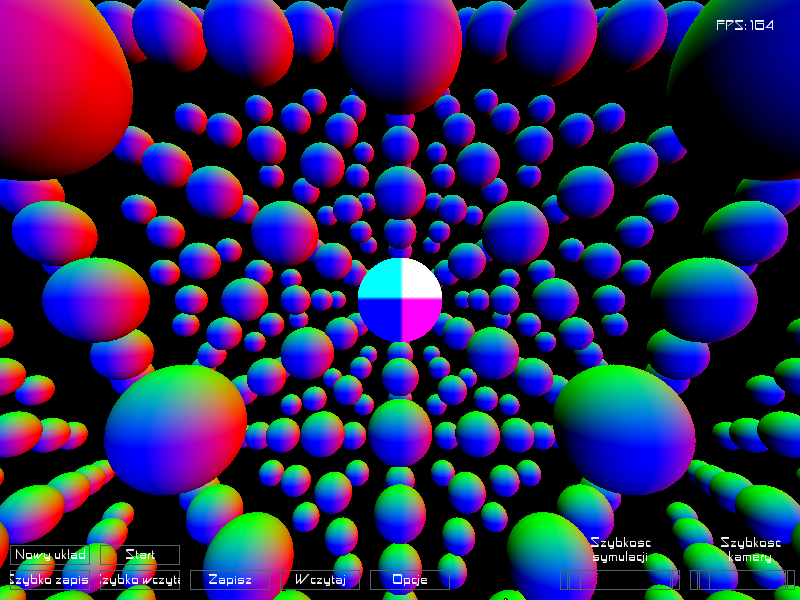
\includegraphics[height=7cm]{img/per2.png}
	\label{fig:per2}
	\end{figure}
	\setcounter{subfigure}{0}
}

\frame
{
	\frametitle{Pozycje}

	\begin{description}
	\item[$pozycja$] -- pozycja powierzchni w danym pikselu
	\item[$normalna$] -- normalna powierzchni w danym pikselu
	\item[$promien$] -- promień planety
	\item[$pozycja\_planety$] -- środek planety
	\end{description}

	$$ pozycja = normalna \cdot promien + pozycja\_planety $$
}

\frame
{
	\frametitle{Pozycje}
	\begin{figure}
	\centering
		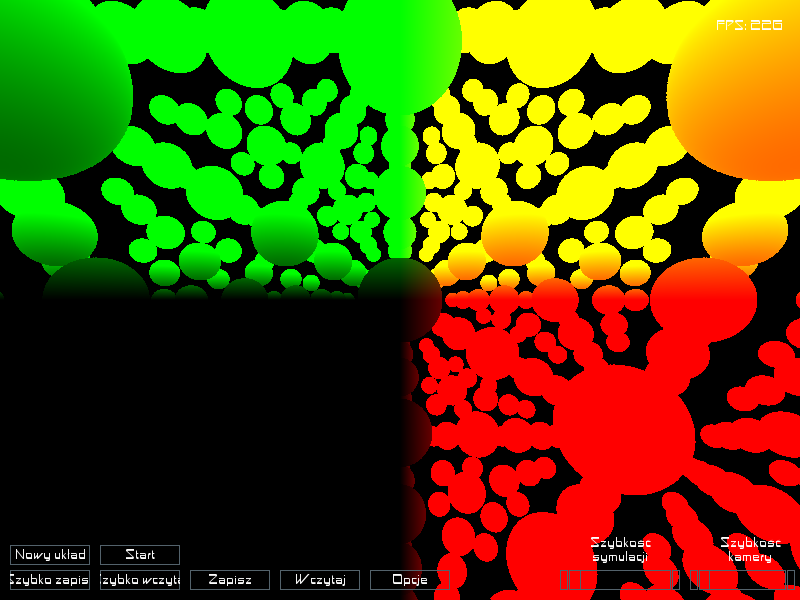
\includegraphics[height=7cm]{img/per3.png}
	\label{fig:per3}
	\end{figure}
	\setcounter{subfigure}{0}
}

\subsection{Oświetlenie}\label{sub:przebieg drugi}
\frame{ \frametitle{Silnik graficzny} \tableofcontents[currentsubsection] }

\frame
{
	\frametitle{Model Phonga}

	\begin{figure}
	\centering
		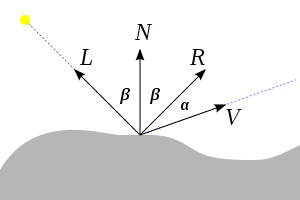
\includegraphics[height=3cm]{img/phong.png}
	\label{fig:phong}
	\end{figure}
	\setcounter{subfigure}{0}
	\begin{description}
	\item[$I_i$] -- natężenie światła padającego
	\end{description}
	$$ I = k_e I_e + k_a I_a + k_d I_d + k_s I_s = k_e I_e + k_a I_a + I_i( k_d( N \cdot L ) + k_s ( R \cdot V )^n ) $$
	\pause $$ I = k_e I_e + k_a I_a + k_d I_d = k_a I_a + I_i k_d( N \cdot L ) $$

}

\frame
{
	\frametitle{Oświetlenie}
	\begin{figure}
	\centering
		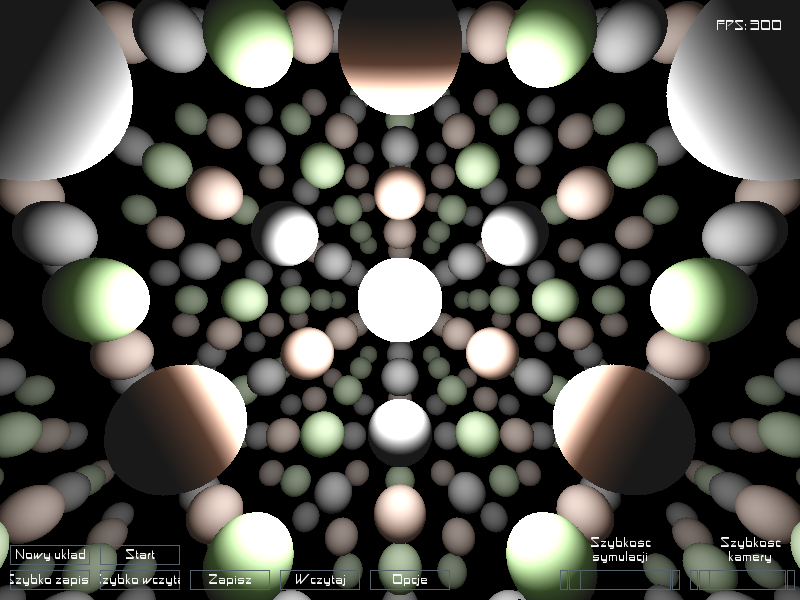
\includegraphics[height=7cm]{img/light0.png}
	\label{fig:per2}
	\end{figure}
	\setcounter{subfigure}{0}
}

\begin{frame}[fragile]
	\frametitle{Addytywność światła}
	$$ I = k_e I_e + k_a I_a + \sum_{i=0}^{lights}{k_{d_i} I_{d_i}} $$
	\pause
	\begin{figure}
	\centering
		\verb| |
		\subfloat[ambient]{\label{fig:lamb}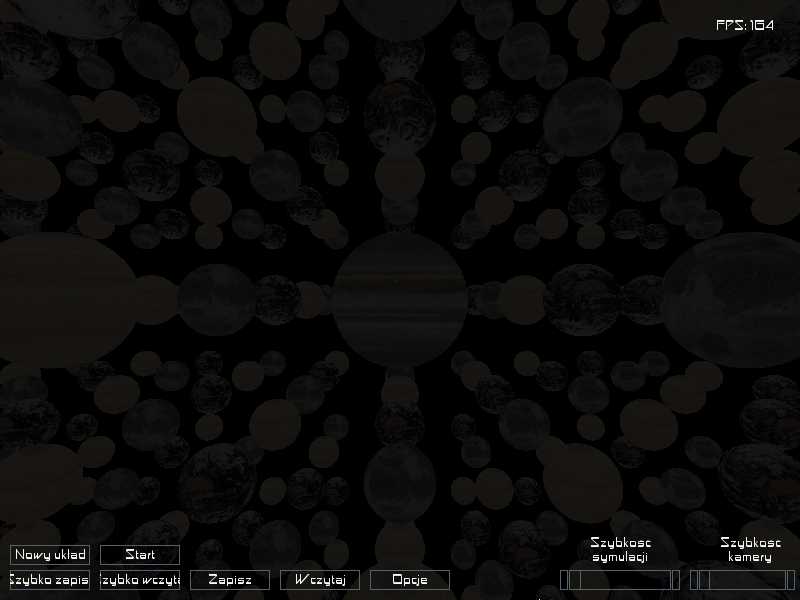
\includegraphics[width=0.30\textwidth]{img/light1.png}} \hspace{.0\textwidth}
		\verb|+|
		\subfloat[diffuse 1]{\label{fig:ldif1}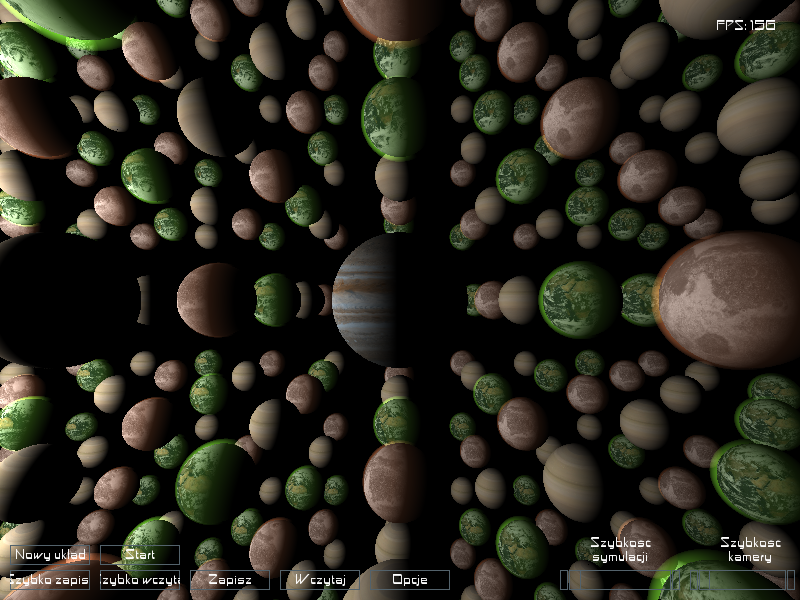
\includegraphics[width=0.30\textwidth]{img/light2.png}} \hspace{.0\textwidth}
		\verb|+|
		\\
		\verb|+|
		\subfloat[diffuse 2]{\label{fig:ldif2}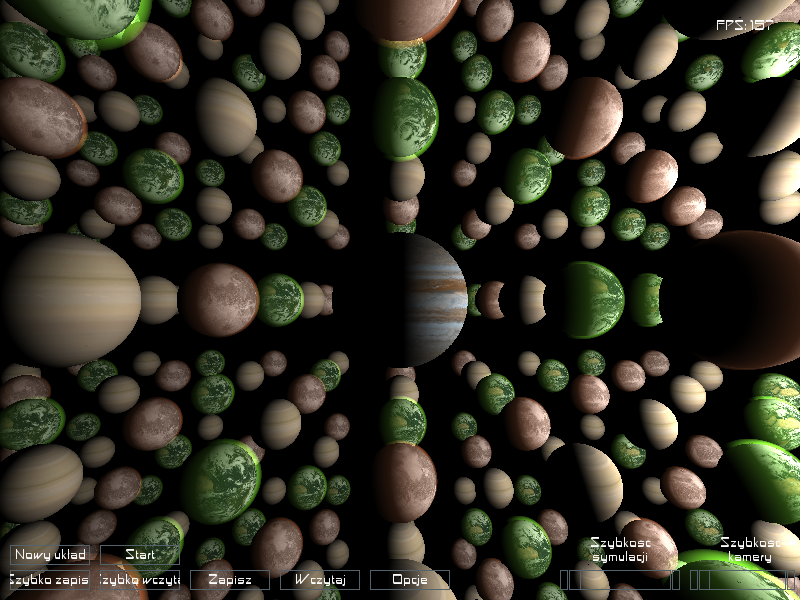
\includegraphics[width=0.30\textwidth]{img/light3.png}} \hspace{.0\textwidth}
		\verb|=|
		\subfloat[efekt]{\label{fig:lend}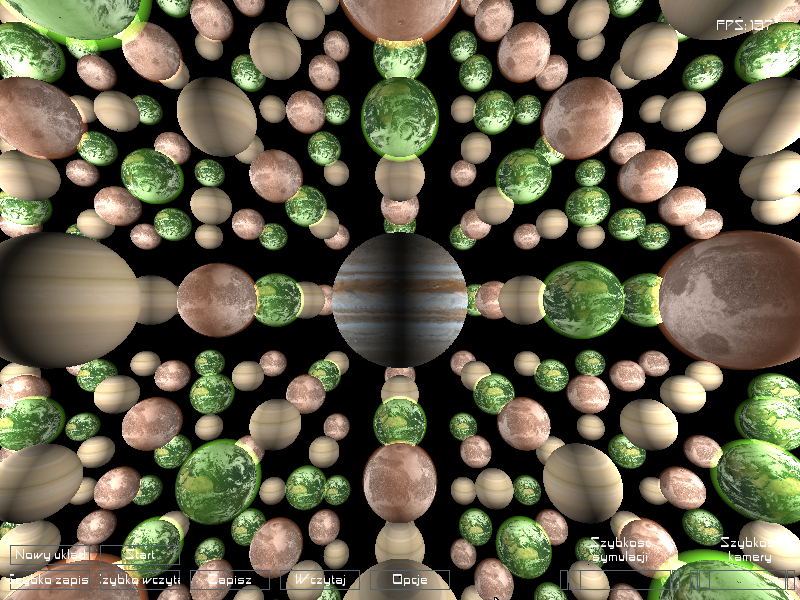
\includegraphics[width=0.30\textwidth]{img/light4.png}}
		\verb| |
	\label{fig:deferred_rednering}
	\end{figure}
	\setcounter{subfigure}{0}
\end{frame}

\subsection{Teksturowanie}\label{sub:teksturowanie}
\frame{ \frametitle{Silnik graficzny} \tableofcontents[currentsubsection] }

\frame
{
	\frametitle{Mapowanie}

	\begin{description}
	\item[UV mapping] -- siatka obiektu na płaszczyźnie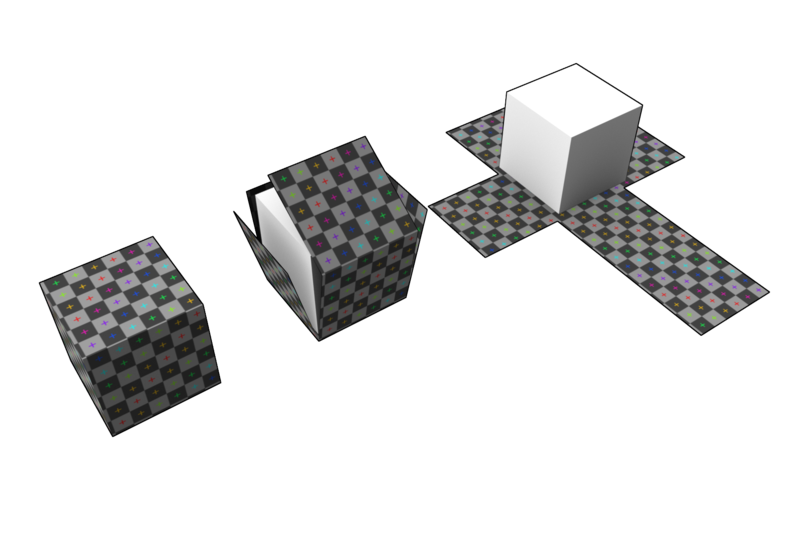
\includegraphics[width=0.30\textwidth]{img/uv_wrapping.png}
	\pause
	\item[Odwzorowania geograficzne] -- odwzorowanie kuli na płaszczyźnie
	\end{description}
}

\frame
{
	\frametitle{Odwzorowania geograficzne}

	\begin{itemize}
	\item Zachowujące kąty
	\item Zachowujące odległość
	\item Zachowujące kierunki
	\item Zachowujące powierzchnię
	\end{itemize}

	\pause

	\begin{figure}
	\centering
	\subfloat[Mercator]{\label{fig:proj_mer}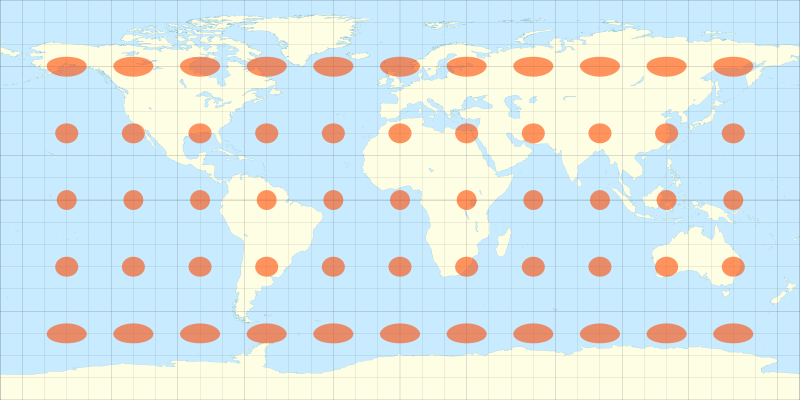
\includegraphics[width=0.45\textwidth]{img/proj_mer.png}} \hspace{.0\textwidth}
	\pause
	\subfloat[Sinusoidalne]{\label{fig:proj_sin}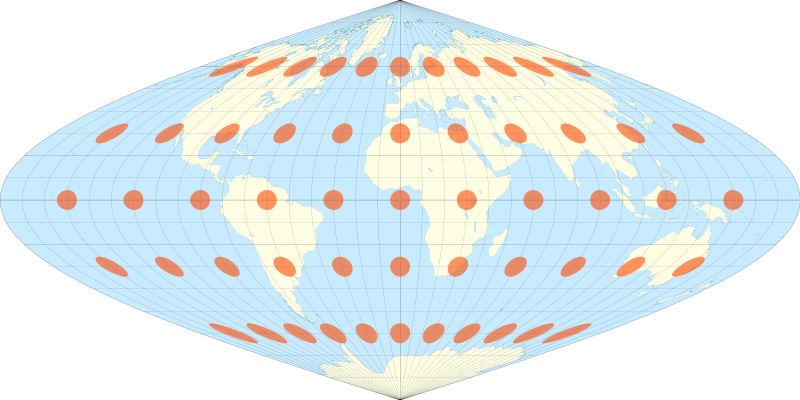
\includegraphics[width=0.45\textwidth]{img/proj_sin.png}}
	\label{fig:normmap}
	\end{figure}
	\setcounter{subfigure}{0}
}

\frame
{
	\frametitle{Przeliczanie koordynat}

	\begin{itemize}
	\item UV tekstury (mapowanie sinusoidalne):
		\begin{eqnarray*}
		u &=& \lambda cos(\phi) \\
		v &=& \phi
		\end{eqnarray*}
	\pause
	\item Współrzędne:
		\begin{eqnarray*}
		\lambda &=& \arctan(\frac{z}{x}) \\
		\phi &=& \arcsin(\frac{y}{r}) = \arcsin(y) 
		\end{eqnarray*}
	\end{itemize}
}

\frame
{
	\frametitle{Zmiana przestrzeni}

	\begin{description}
	\item[Przestrzeń kamery] -- (0,0,0) w miejscu kamery
	\item[Przestrzeń obiektu] -- (0,0,0) w środku planety
	\end{description}

	\pause

	\begin{description}
	\uncover<2->{
	\item[$N$] -- normalna 
	\item[$R$] -- macierz rotacji
	} \uncover<4-> {
	\item[$K$] -- macierz przekształcenia kamery
	}
	\end{description}
	\begin{eqnarray*}
	\uncover<2->{
	(x,y,z) &=& R \cdot N \\
	} \uncover<3->{
	R &=& R_k^T \\
	} \uncover<5->{
	R_k &=& 
	\left| \begin{array}{cccc}
	K_{11} & K_{12} & K_{13} & 0 \\
	K_{21} & K_{22} & K_{23} & 0 \\
	K_{31} & K_{32} & K_{33} & 0 \\
	0 & 0 & 0 & 1 
	\end{array} \right|
	}
	\end{eqnarray*}
}

\frame
{
	\frametitle{Tekstury}
	\begin{figure}
	\centering
		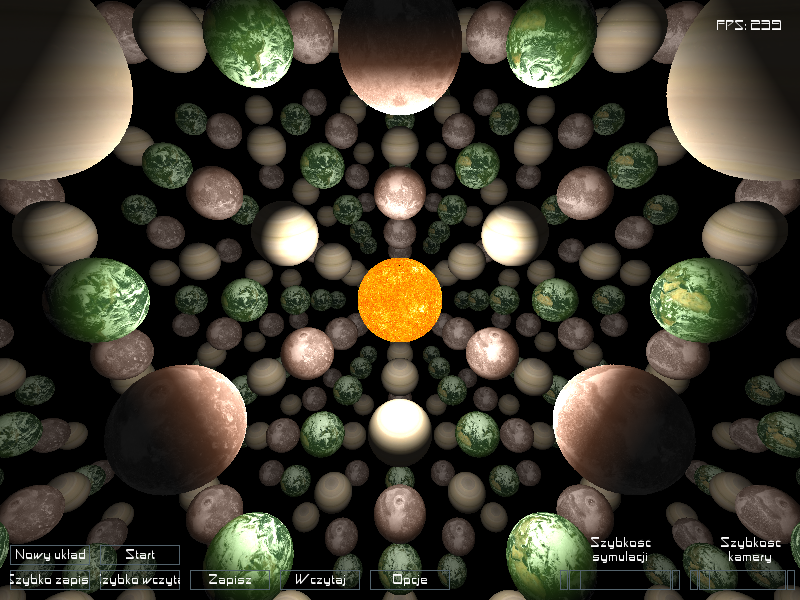
\includegraphics[height=7cm]{img/per4.png}
	\label{fig:per4}
	\end{figure}
}

%\subsection{Atmosfery}\label{sub:atmosfery}
%\frame{ \frametitle{Silnik graficzny} \tableofcontents[currentsubsection] }

%\section{Picking}\label{sec:picking}

\section{Silnik fizyczny}
\subsection{Reprezentacja klastrów}

\frame
{
	\frametitle{Fizyka}
	\tableofcontents[currentsubsection]
}

\frame
{
	\frametitle{Reprezentacja klastrów}
	\begin{figure}
	\centering
		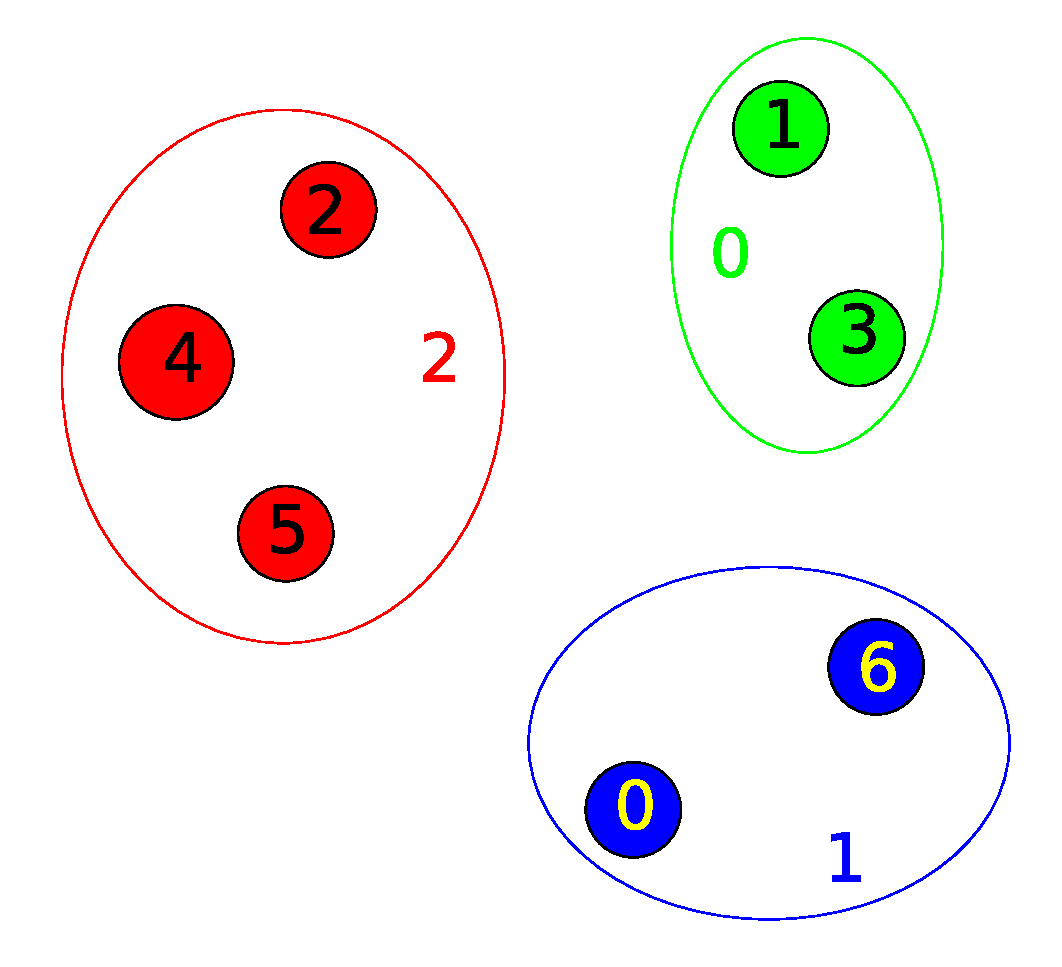
\includegraphics[height=5cm]{img/clusters.pdf}
	\end{figure}
	\setcounter{subfigure}{0}
}

\frame
{
	\frametitle{shuffle i count}
	\begin{figure}
		\centering
		Count: \\
		\begin{tabular}{|c|c|c|}
		\hline
		0 & 1 & 2 \\
		\hline
		2 & 5 & 7 \\
		\hline
		\end{tabular} \\
		\pause
		\vspace{1cm}
		Shuffle: \\
		\begin{tabular}{|c|c||c|c|c||c|c|}
		\hline
		0 & 1 & 2 & 3 & 4 & 5 & 6 \\
		\hline
		1 & 3 & 2 & 4 & 5 & 0 & 6 \\
		\hline
		\end{tabular} \\
	\end{figure}
}

\subsection{Usuwanie planet}

\frame
{
	\frametitle{Usuwanie planet}
	\begin{figure}
		\centering
		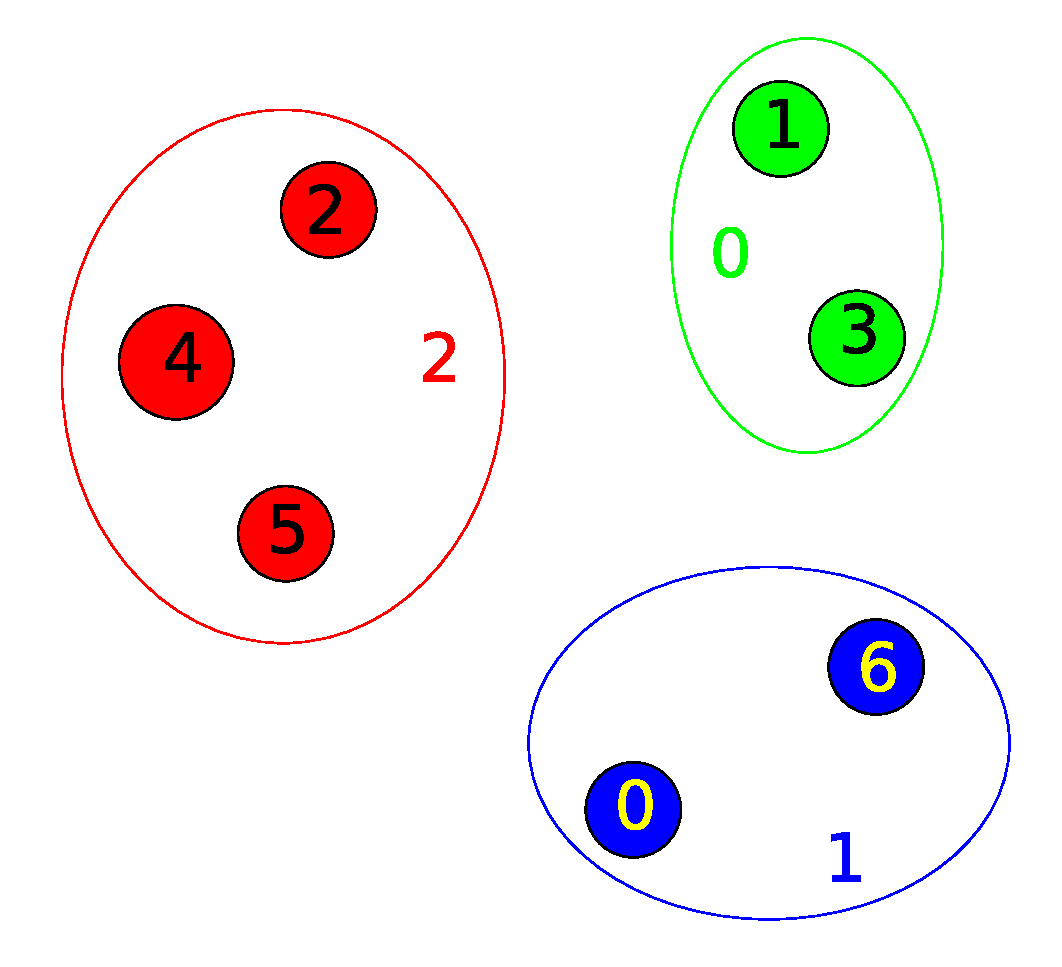
\includegraphics[height=5cm]{img/clusters.pdf}
	\end{figure}
	\setcounter{subfigure}{0}
}

\frame
{
	\frametitle{Usuwanie planet}
	\begin{figure}
		\centering
		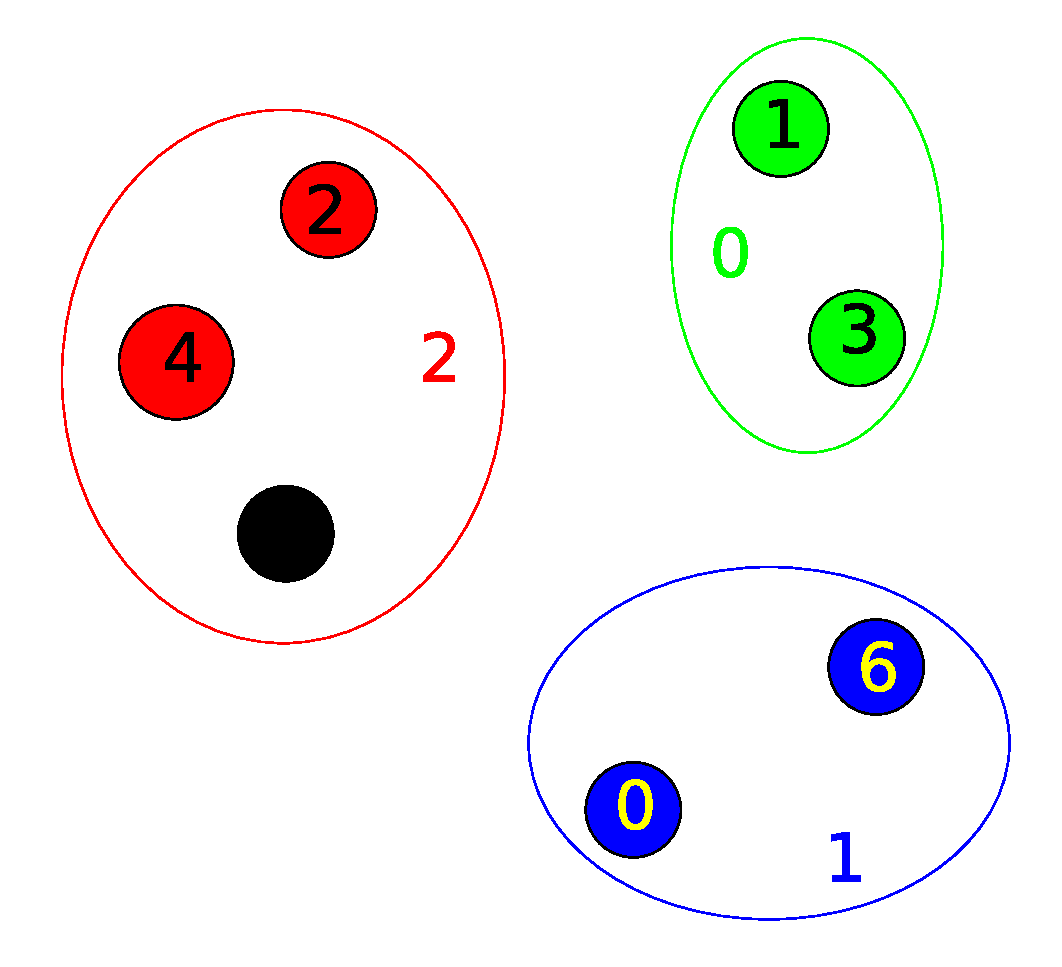
\includegraphics[height=5cm]{img/clusters2.pdf}
	\end{figure}
	\setcounter{subfigure}{0}
}

\frame
{
	\frametitle{Usuwanie planet}
	Rodzaje:
	\begin{itemize}
	\item Usuniecie logiczne
	\item Usunięcie fizyczne
	\end{itemize}
}

\frame
{
	\frametitle{Usunięcie logiczne}
	\begin{itemize}
		\item dla grafiki:
		\begin{itemize}
			\item{Obiekty zerowych rozmiarów są niewidoczne}
			\item{promień = 0}
		\end{itemize}
		\item dla fizyki:
		\begin{itemize}
			\item{Obiekty o zerowej masie nie wpływają na inne}
		\end{itemize}
		\hspace{0.6cm}
		$$ \overrightarrow{F_1} = G\frac{m_1 m_2}{r^2}\overrightarrow{e_{12}}  $$
		$$ \overrightarrow{a_1}m_1 = G\frac{m_1 m_2}{r^2}\overrightarrow{e_{12}}  $$
		$$ \overrightarrow{a_1} = G\frac{m_2}{r^2}\overrightarrow{e_{12}}  $$
	\end{itemize}
}

\frame
{
	\frametitle{Usunięcie fizyczne}
	\begin{itemize}
	\item{cudppCompact}
	\item{cudppScan + Compacter}
	\end{itemize}
}

\subsection{Kolizje}

\frame
{
	\frametitle{Podział akcji}
	\begin{itemize}
		\item Detekcja kolizji
		\item Obsługa kolizji
	\end{itemize}
}

\begin{frame}[fragile]
	\frametitle{Algorytm detekcji kolizji}

	\begin{verbatim}
foreach planet p in parallel
   id = p.index + 1
   while id < count[ p.cluster ]
      if( kolizja( p, planet[ shuffle[ id ] ] ) )
         k[ shuffle[ p.id ] ] = shuffle[ id ]
         return;
      ++id
   k[ shuffle[ p.id ] ] = shuffle[ p.id ]
	\end{verbatim}
\end{frame}

\begin{frame}[fragile]
	\frametitle{Algorytm obsługi kolizji}
	\begin{verbatim}
done = false
k_in = k
while !done
   done = true
   foreach planet p in parallel   
      if( k_in[ p.id ] == p.id )
         k_out[ p.id ] = p.id
         return
      if( k_in[ k_in[ p.id ] ] != k_in[ p.id ] )
         k_out[ p.id ] = k_in[ p.id ]
         done = false
      merge( p, planet[ k_in[ p.id ] ] )
      k_out[ p.id ] = p.id
   k_in <=> k_out
   \end{verbatim}
\end{frame}

\frame
{
	\frametitle{Koniec}
	\begin{figure}
		\centering Dziękujemy za uwagę
	\end{figure}
	\setcounter{subfigure}{0}
}

\end{document}


